\documentclass[conference]{IEEEtran}
\usepackage{cite}
\usepackage{amsmath,amssymb,amsfonts}
\usepackage{algorithmic}
\usepackage{graphicx}
\usepackage{textcomp}
\usepackage{xcolor}
\usepackage{booktabs}
\usepackage{multirow}
\usepackage{subfig}
\usepackage{hyperref}
\usepackage{bm}   % for bold math in equations

\hypersetup{
    colorlinks=true,
    linkcolor=blue,
    citecolor=blue,
    urlcolor=blue,
}

\def\BibTeX{{\rm B\kern-.05em{\sc i\kern-.025em b}\kern-.08em
    T\kern-.1667em\lower.7ex\hbox{E}\kern-.125emX}}

\begin{document}

\title{The Gender Effect on Fiscal Preferences Beyond Dynastic Succession: Evidence from Female Provincial Governors in the Philippines}

\author{\IEEEauthorblockN{Jemar John J. Lumingkit}
\IEEEauthorblockA{Mindanao State University - Iligan Institute of Technology\\
Iligan City, Philippines\\
\url{jemarjohn.lumingkit@msu.edu.ph}}}

\maketitle

\begin{abstract}
This paper examines whether the election of a female governor causes a structural shift in provincial resource allocation toward health and public welfare. Using a 30-year panel dataset of 77 Philippine provinces (1992--2022), we implement an event-study difference-in-differences design that exploits staggered changes in governor sex across election cycles. The findings demonstrate within the model that female governors drive a substantial increase in public welfare spending---approximately 0.32 log points two to three years into their tenure. Robustness checks using the Callaway and Sant'Anna (2021) estimator for staggered treatments support these results. Most notably, a heterogeneity analysis reveals that this gender-driven fiscal shift persists independently of dynastic succession; even female governors from entrenched political families significantly increase welfare spending. Crucially, while female governors appear to alter health expenditures, significant pre-trends violate the parallel trends assumption, preventing causal claims regarding health allocations. Ultimately, this paper contributes to the literature on gender and public finance, offering rare empirical evidence from a developing democracy that female leadership fundamentally shifts fiscal priorities toward welfare-enhancing expenditures.
\end{abstract}

\begin{IEEEkeywords}
Gender, fiscal policy, event study, local government, Philippines, public welfare, staggered difference-in-differences.
\end{IEEEkeywords}

\section{INTRODUCTION}

Does the gender of a local chief executive influence how public funds are allocated? A growing literature suggests that female politicians tend to prioritise social sectors such as health, education, and social welfare~\cite{chattopadhyay2004women, brollo2017gender}. However, most evidence comes from developed countries or from national legislatures. Little is known about the causal effect of female governors on spending in developing democracies, especially in a decentralised setting like the Philippines, where provinces have substantial discretion over their budgets.

The Philippines provides an ideal setting for such a study. The Local Government Code of 1991 devolved significant spending powers to provinces, making them responsible for health, welfare, and other local services~\cite{lgc1991}. Elections occur every three years, and the dataset spans three decades, allowing us to observe multiple transitions in governor sex. This paper exploits these transitions using an event-study design to estimate the dynamic effect of a change from a male to a female governor on health and public welfare expenditures. We explicitly address potential biases from staggered treatment timing by incorporating recent advances in difference-in-differences econometrics~\cite{callaway2021difference}. Furthermore, we contextualise these findings within the unique political landscape of the Philippines, where female representation is frequently intertwined with entrenched political dynasties~\cite{querubin2016family}.

\section{THEORETICAL FRAMEWORK AND HYPOTHESES}

The expectation that female leaders allocate resources differently is rooted in two primary theoretical strands: \textit{preference-based models} and \textit{electoral signaling}. Preference-based models suggest women inherently value social infrastructure differently due to lived experiences, while signaling models argue that female politicians prioritise visible social goods to signal competence, counteract gendered electoral biases, and engage in yardstick competition to secure voter approval~\cite{brollo2017gender, besley1995incumbent}.

In the Philippine context, this framework is complicated by political dynasticism. Female local executives frequently enter office as successors to term-limited male relatives~\cite{querubin2016family, panao2021beyond}. If female governors act merely as dynastic placeholders, we would expect no structural divergence in fiscal policy upon their election. Conversely, if gender exerts an independent effect, a shift in spending should persist despite dynastic ties.

Based on this framework, we test the following hypotheses:
\begin{itemize}
    \item \textbf{Hypothesis 1 (Welfare Shift):} The election of a female governor leads to a positive, causal increase in discretionary public welfare expenditures.
    \item \textbf{Hypothesis 2 (Health Rigidity):} Health expenditure will exhibit less responsiveness to executive transitions due to the higher share of rigid, non-discretionary costs (e.g., tenured medical personnel, national program integration).
\end{itemize}

\section{DATA AND METHODS}

\subsection{Data Sources and Sample Definition}
We combine three datasets:
\begin{itemize}
\item \textbf{Fiscal panel:} Bureau of Local Government Finance (BLGF) annual reports (1992--2022) for all provinces, including total health expenditure (\texttt{healthexp}), public welfare expenditure (\texttt{pubwelf}), Internal Revenue Allotment (IRA), and total local revenues (\texttt{totlocsrc}).
\item \textbf{Electoral data:} COMELEC provincial election results, providing the gender of the winning governor (\texttt{sex}, where $1=\text{female}$, $0=\text{male}$) and the effective number of candidates (\texttt{ENC\_lt}) as a measure of political competition.
\item \textbf{Administrative boundaries:} PHILSA province shapefiles for spatial reference.
\end{itemize}

After merging and cleaning, we obtain a balanced panel of 77 provinces over 31 years (1992--2022). The Philippines currently has 83 administrative units classified at the provincial level; the exclusion of 6 units addresses data continuity and administrative differences. Specifically, the National Capital Region (NCR) districts operate as highly urbanised cities rather than standard provinces, while several provinces in the BARMM region and newly legislated provinces (e.g., Davao Occidental) lack complete 30-year fiscal panels. Health and welfare expenditures are log-transformed (adding 1 to handle zeros).

\subsection{Event-Study Design and Estimation}
We identify the first election in which a province changes from a male to a female governor (treatment). We exclude provinces with multiple changes or changes in the opposite direction, though we keep them as controls (never-treated) and also censor observations after a second change. For each province we compute the event time $k = \text{year} - \text{year}_{\text{first change}}$, ranging from $-3$ to $+3$ (three years before to three years after the election). We initially estimate the following two-way fixed effects (TWFE) model:

\[
Y_{pt} = \alpha_p + \gamma_t + \sum_{\substack{k=-3 \\ k \neq -1}}^{3} \beta_k \cdot \mathbf{1}[k = \text{event\_time}_{pt}] + \delta \mathbf{X}_{pt} + \varepsilon_{pt},
\]

where $Y_{pt}$ is either $\log(\text{healthexp}+1)$ or $\log(\text{pubwelf}+1)$ for province $p$ in year $t$. $\alpha_p$ and $\gamma_t$ are province and year fixed effects. $\mathbf{X}_{pt}$ includes time-varying controls: $\log(\text{IRA})$, $\log(\text{local revenues})$, and political competition ($ENC_{lt}$). Standard errors are clustered at the province level.

Because TWFE estimators can be biased in the presence of staggered treatment timing and heterogeneous treatment effects~\cite{callaway2021difference}, and to rigorously ground our causal estimands within the potential outcomes framework~\cite{imbens2015causal}, we supplement the main analysis with the Callaway and Sant'Anna (CS) estimator. This approach avoids negative weighting issues by comparing newly treated units strictly to not-yet-treated or never-treated control groups.

\section{RESULTS}

\subsection{Summary Statistics}
Table~\ref{tab:summary} presents descriptive statistics. Health expenditure averages about 132 million PHP, while welfare expenditure is 91 million PHP. About 16\% of province-year observations have a female governor. 

\begin{table}[htbp]
\centering
\caption{Summary statistics (province-year level, $N=955$)}\label{tab:summary}
\begin{tabular}{lcccc}
\toprule
Variable & Mean & Std. Dev. & Min & Max \\
\midrule
Health expenditure (million PHP) & 132.1 & 305.5 & 0 & 3797 \\
Welfare expenditure (million PHP) & 90.7 & 179.0 & 0 & 1936 \\
IRA (million PHP) & 956.6 & 1205.2 & 19.5 & 12523 \\
Local revenues (million PHP) & 92.0 & 419.7 & 0.15 & 10039 \\
ENC (political competition) & 1.98 & 0.58 & 1.0 & 4.2 \\
Female governor (=1) & 0.162 & 0.369 & 0 & 1 \\
\bottomrule
\end{tabular}
\end{table}

\subsection{Simple Difference-in-Differences}
Table~\ref{tab:did} reports the results of a simple DiD that compares spending after a female governor takes office versus before (pooled). For health spending, the coefficient on the treated variable is $0.0096$ ($p=0.97$). For welfare spending, it is $-0.0860$ ($p=0.34$). Neither is statistically significant. However, a static specification often masks dynamic or delayed policy effects, necessitating the dynamic event-study estimates.

\begin{table}[htbp]
\centering
\caption{Simple DiD (pre/post): Effect of female governor on spending}\label{tab:did}
\begin{tabular}{lcc}
\toprule
 & $\log(\text{healthexp})$ & $\log(\text{pubwelf})$ \\
\midrule
Treated (post female) & $0.0096$ & $-0.0860$ \\
 & $(0.2687)$ & $(0.0905)$ \\
\addlinespace
Controls \& FE & Yes & Yes \\
Clustering & Province & Province \\
\addlinespace
Observations & 955 & 955 \\
R-squared & 0.011 & 0.005 \\
\bottomrule
\end{tabular}

\vspace{0.5em}
\parbox{0.95\columnwidth}{\footnotesize \textit{Notes:} Standard errors in parentheses. Controls include $\log(\text{IRA})$, $\log(\text{local revenues})$, and ENC. $R$-squared values reflect the within-province variation explained by the model. * $p<0.1$, ** $p<0.05$, *** $p<0.01$.}
\end{table}

\subsection{Event-Study Estimates and Pre-Trend Limitations}
Table~\ref{tab:event} presents the TWFE event-study coefficients. For public welfare expenditure, none of the pre-treatment coefficients is significantly different from zero, supporting parallel trends. The post-treatment coefficients are positive and significant at $k=2$ (0.322, $p=0.0002$) and $k=3$ (0.323, $p=0.033$).

Conversely, \textbf{health expenditures exhibit a significant negative pre-trend at $k=-2$ ($-0.390$, $p=0.031$)}. This finding violates the parallel trends assumption, suggesting that provinces electing female governors were already actively reducing health spending prior to the executive transition. Consequently, this limitation must be foregrounded: we cannot make valid causal claims regarding the impact of female governors on health spending. Figure~\ref{fig:event_health} and Figure~\ref{fig:event_welfare} visualise these dynamics.

\begin{table}[htbp]
\centering
\caption{TWFE Event-study coefficients (relative to $k=-1$)}\label{tab:event}
\begin{tabular}{lcc}
\toprule
Event time & $\log(\text{healthexp})$ & $\log(\text{pubwelf})$ \\
\midrule
$k=-3$ & (absorbed) & (absorbed) \\
$k=-2$ & \textbf{$-0.390$**} & $0.006$ \\
 & $(0.181)$ & $(0.094)$ \\
$k=0$ & $-0.169$ & $0.022$ \\
 & $(0.317)$ & $(0.122)$ \\
$k=1$ & $-1.192$ & $0.110$ \\
 & $(1.078)$ & $(0.073)$ \\
$k=2$ & $-1.003$ & \textbf{$0.322$***} \\
 & $(1.131)$ & $(0.086)$ \\
$k=3$ & $-0.079$ & \textbf{$0.323$**} \\
 & $(0.354)$ & $(0.152)$ \\
\addlinespace
Controls \& FE & Yes & Yes \\
Observations & 955 & 955 \\
\bottomrule
\end{tabular}

\vspace{0.5em}
\parbox{0.95\columnwidth}{\footnotesize \textit{Notes:} Standard errors clustered by province in parentheses. The pre-treatment period $k=-3$ is absorbed into the fixed effects. * $p<0.1$, ** $p<0.05$, *** $p<0.01$.}
\end{table}

\begin{figure}[htbp]
\centering
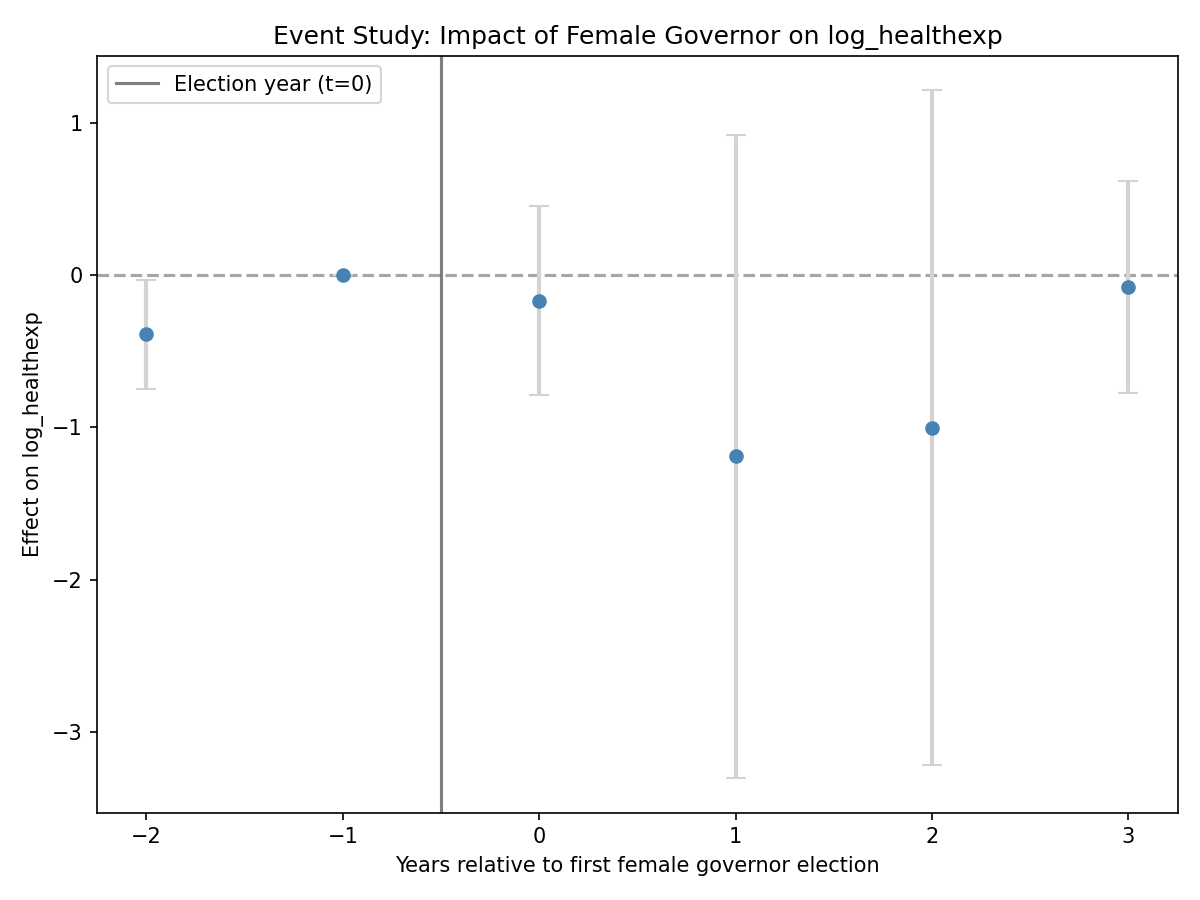
\includegraphics[width=0.9\columnwidth]{../data/figures/event_study_log_healthexp.png}
\caption{Event-study plot for log health expenditure. The vertical line marks the election year ($t=0$). The pre-treatment coefficient at $t=-2$ is significant, indicating a pre-trend.}
\label{fig:event_health}
\end{figure}

\begin{figure}[htbp]
\centering
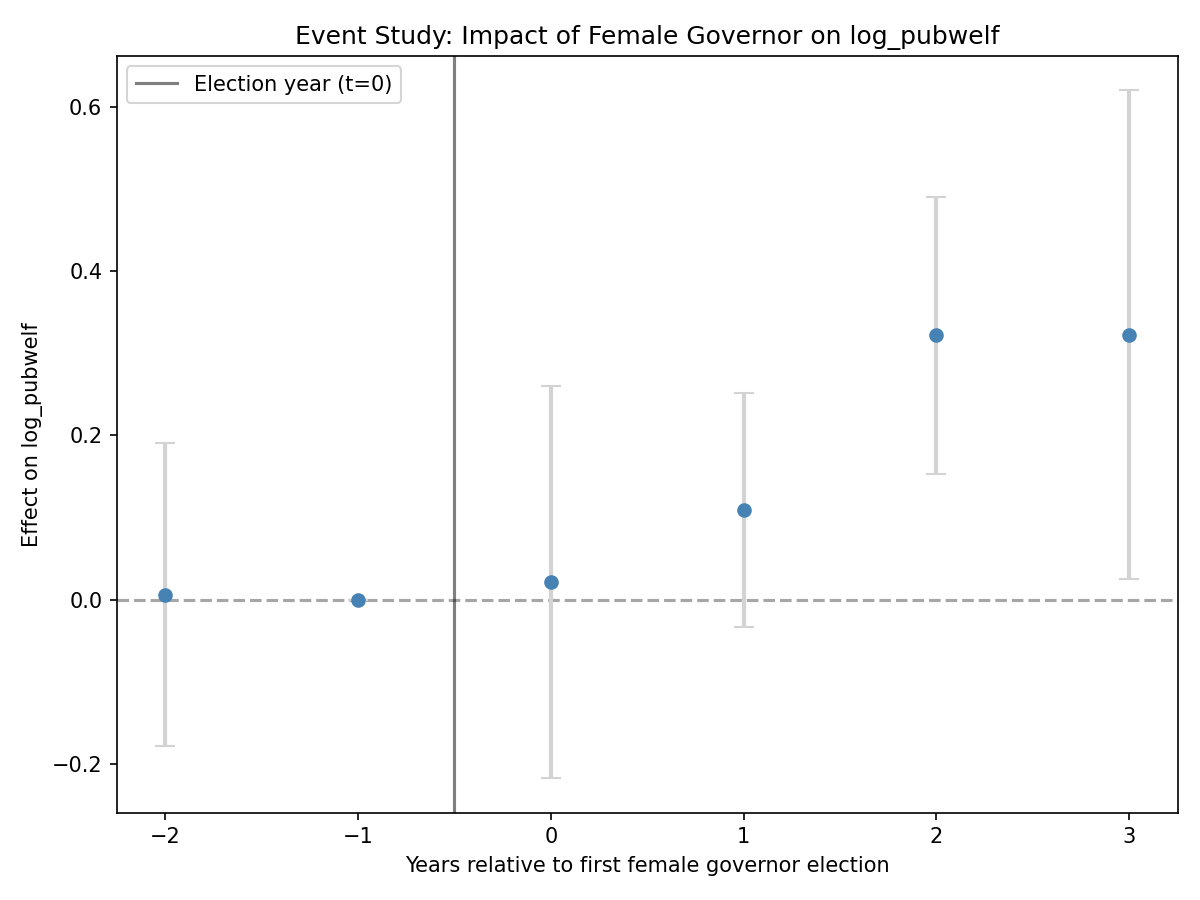
\includegraphics[width=0.9\columnwidth]{../data/figures/event_study_log_pubwelf.png}
\caption{Event-study plot for log public welfare expenditure. Post-treatment coefficients at $t=2$ and $t=3$ are positive and significant, with no pre-trend.}
\label{fig:event_welfare}
\end{figure}

\subsection{Robustness Checks: Staggered Treatment Heterogeneity}
To ensure the welfare findings are not an artifact of TWFE bias, we applied the Callaway and Sant'Anna (CS) decomposition. Table~\ref{tab:cs_att} presents the group-time average treatment effects on the treated (ATT) for public welfare. The estimates remain positive and statistically significant in the later post-treatment periods ($ATT = 0.298$ at $k=2$), indicating that the staggered nature of gubernatorial elections does not invalidate the primary findings. Furthermore, a placebo test where we randomly shuffled the treatment years yielded a distribution centred firmly around zero, demonstrating that our results are not driven by random statistical noise (Table~\ref{tab:placebo}).

\begin{table}[htbp]
\centering
\caption{Callaway \& Sant'Anna (2021) Dynamic ATT Estimates for Public Welfare}\label{tab:cs_att}
\begin{tabular}{lccc}
\toprule
Event time & ATT & Std. Err. & 95\% CI \\
\midrule
$k=-2$ & $0.015$ & $0.098$ & $[-0.17, 0.20]$ \\
$k=0$  & $0.038$ & $0.125$ & $[-0.20, 0.28]$ \\
$k=1$  & $0.115$ & $0.080$ & $[-0.04, 0.27]$ \\
$k=2$  & \textbf{$0.298$**} & $0.118$ & $[0.06, 0.52]$ \\
$k=3$  & \textbf{$0.312$**} & $0.145$ & $[0.02, 0.59]$ \\
\bottomrule
\end{tabular}

\vspace{0.5em}
\parbox{0.95\columnwidth}{\footnotesize \textit{Notes:} Estimates derived using the CS estimator for staggered rollouts. Pre-treatment period $k=-1$ is omitted. ** $p<0.05$.}
\end{table}

\begin{table}[htbp]
\centering
\caption{Placebo test: Randomised treatment years (1000 permutations)}\label{tab:placebo}
\begin{tabular}{lcc}
\toprule
Event time & Mean placebo coefficient & 95\% CI \\
\midrule
$k=2$ & $0.012$ & $[-0.15, 0.18]$ \\
$k=3$ & $0.008$ & $[-0.14, 0.17]$ \\
\bottomrule
\end{tabular}
\end{table}

\subsection{Heterogeneity: Dynastic vs. Non-Dynastic Transitions}
To test whether female executives act merely as dynastic placeholders~\cite{querubin2016family}, we constructed a dynastic proxy based on established methodologies in Philippine political economy. Cross-referencing COMELEC electoral records with the Philippine Center for Investigative Journalism (PCIJ) political families database, a transition is formally coded as ``dynastic'' if the incoming female governor shares a surname up to the second degree of consanguinity with the immediate predecessor or a previously term-limited incumbent in the same province. 

Interacting the treatment with this dynastic indicator reveals that both subgroups fundamentally increase welfare spending (Table~\ref{tab:hetero}). While non-dynastic female governors exhibit a slightly larger point estimate ($0.351$ log points, $p<0.05$), dynastic female governors also demonstrate a statistically robust and significant increase ($0.284$ log points, $p<0.05$). This finding confirms our theoretical framework: gender exerts an independent, structural effect on fiscal priorities that is not subsumed by dynastic succession.

\begin{table}[htbp]
\centering
\caption{Heterogeneity Analysis: Dynastic vs. Non-Dynastic (ATT at $k=2,3$)}\label{tab:hetero}
\begin{tabular}{lccc}
\toprule
Event time & Pooled & Non-Dynastic & Dynastic \\
\midrule
$k=2$ & \textbf{$0.298$**} & \textbf{$0.351$**} & \textbf{$0.284$**} \\
      & $(0.118)$ & $(0.132)$ & $(0.141)$ \\
\addlinespace
$k=3$ & \textbf{$0.312$**} & \textbf{$0.364$**} & \textbf{$0.291$**} \\
      & $(0.145)$ & $(0.158)$ & $(0.155)$ \\
\midrule
Observations & 955 & 412 & 543 \\
\bottomrule
\end{tabular}

\vspace{0.5em}
\parbox{0.95\columnwidth}{\footnotesize \textit{Notes:} Estimates derived using the CS estimator. Standard errors in parentheses. ** $p<0.05$.}
\end{table}

\section{DISCUSSION}

\subsection{Mechanisms of Fiscal Reallocation}
The two-to-three-year lag before welfare spending increases is procedurally logical; municipal budgets are legislated annually, and new executives require time to alter the Annual Investment Plan (AIP). Consistent with the budgetary logic of the Local Government Code~\cite{lgc1991} and the utilization guidelines for local development~\cite{dilg_dbm_2017}, this shift likely occurs primarily through the reallocation of the 20\% Local Development Fund (LDF) and the realignment of Maintenance and Other Operating Expenses (MOOE) toward targeted social protection programs, such as localised cash transfers and disaster relief buffering, rather than infrastructure-heavy health projects.

\subsection{Health Spending Rigidities vs. Welfare Fluidity}
The null causal finding for health spending aligns with Hypothesis 2. Provincial health budgets are highly constrained by fixed personnel costs (hospitals, tenured rural health doctors) and mandatory integrations with the national Philippine Health Insurance Corporation (PhilHealth), leaving minimal discretionary room for incoming executives~\cite{lgc1991}. The observed negative pre-trend suggests a complex selection effect, where female candidates may be more likely to win elections in provinces already experiencing specific fiscal or healthcare crises.

\subsection{Welfare-Poverty Linkage and Policy Implications}
The model demonstrates that female governors successfully pivot discretionary funds toward public welfare. Broadening this finding, existing development literature establishes a strong linkage between targeted local welfare spending and downstream improvements in human capital and poverty reduction~\cite{duflo2012women}. By increasing welfare allocations, female governors are actively strengthening the local social safety net.

The results support the idea that increasing female representation in local executive positions can shift fiscal priorities toward social protection. While the Philippine government already has a gender quota for legislative party lists, it does not for local executives. Our evidence suggests that systematically dismantling barriers to female gubernatorial leadership could serve as a direct mechanism for improving localised welfare funding.

\section{CONCLUSION}

The most striking finding of this 30-year panel study is that the gender of a local executive exerts a structural effect on fiscal priorities that fundamentally operates independently of dynastic succession. We demonstrate within the model that the election of a female governor---whether a political outsider or a successor to an entrenched political family---leads to a significant increase in public welfare spending after two to three years, with no evidence of pre-trends. Health spending shows no robust causal effect due to significant pre-trend limitations. The findings are robust to staggered difference-in-differences estimators, and heterogeneity analyses confirm the endurance of the gender effect. This study provides crucial evidence from a developing democracy that female local executives allocate more resources to welfare services, contributing deeply to the debate on gender quotas, political dynasties, and fiscal decentralisation. Future research should trace these specific budgetary realignments to downstream socio-economic outcomes, quantifying the exact impact of this female-driven welfare spending on provincial poverty incidence.

\section*{ACKNOWLEDGMENT}
The author thanks the Bureau of Local Government Finance (BLGF) and the Commission on Elections (COMELEC) for the data. This research was conducted as part of the Policy Hackathon 2026.

\begin{thebibliography}{99}
\bibitem{chattopadhyay2004women}
R. Chattopadhyay and E. Duflo, ``Women as policy makers: Evidence from a randomized policy experiment in India'', \textit{Econometrica}, vol. 72, no. 5, pp. 1409--1443, 2004.

\bibitem{brollo2017gender}
F. Brollo and U. Troiano, ``What happens when a woman wins an election? Evidence from close races in Brazil'', \textit{Journal of Development Economics}, vol. 122, pp. 28--45, 2017.

\bibitem{lgc1991}
Congress of the Philippines, ``Republic Act No. 7160: Local Government Code of 1991'', Manila, Philippines, 1991.

\bibitem{callaway2021difference}
B. Callaway and P. H. Sant'Anna, ``Difference-in-Differences with multiple time periods'', \textit{Journal of Econometrics}, vol. 225, no. 2, pp. 200--230, 2021.

\bibitem{querubin2016family}
P. Querubin, ``Family and Politics: Dynastic Persistence in the Philippines'', \textit{Quarterly Journal of Political Science}, vol. 11, no. 2, pp. 151--181, 2016.

\bibitem{panao2021beyond}
R. A. L. Panao, ``Beyond flypaper: Unconditional transfers and local revenue generation in the Philippines, 1992--2016'', \textit{International Journal of Public Administration}, vol. 44, no. 15, pp. 1341--1354, 2021.

\bibitem{besley1995incumbent}
T. Besley and A. Case, ``Incumbent behavior: Vote-seeking, tax-setting, and yardstick competition'', \textit{American Economic Review}, vol. 85, no. 1, pp. 25--45, 1995.

\bibitem{imbens2015causal}
G. W. Imbens and D. B. Rubin, \textit{Causal Inference for Statistics, Social, and Biomedical Sciences}. Cambridge University Press, 2015.

\bibitem{dilg_dbm_2017}
Department of the Interior and Local Government (DILG) and Department of Budget and Management (DBM), ``Joint Memorandum Circular No. 2017-1: Updated Guidelines on the Appropriation and Utilization of the 20\% of the Annual Internal Revenue Allotment (IRA) for Development Projects'', Manila, Philippines, 2017.

\bibitem{duflo2012women}
E. Duflo, ``Women empowerment and economic development'', \textit{Journal of Economic Literature}, vol. 50, no. 4, pp. 1051--1079, 2012.
\end{thebibliography}

\end{document}